\subsection{Overview}
The basic architecture of our SyncSpecCNN is similar to the fully convolutional segmentation network as in \cite{long2015fully}, namely, we repeat the operation of convolving the vertex function by kernels and applying non-linear transformation. However, we have several key differences. First, we achieve convolution by modulation in the spectral domain.
%To be specific, we first transform a vertex function to its spectral representation, then modulate this representation by a set of learnable multipliers, and finally transform the spectral representation back to obtain the convolved vertex function. The multipliers essentially defines the set of convolution kernels. 
Second, we parametrize kernels in the spectral domain following a dilated fashion, so that kernel sizes could be effectively enlarged to capture large context information without increasing the number of parameters.
%Large kernels have been proved to be very helpful for image segmentation tasks due to its ability of effectively capturing large context information \cite{yu2015multi}. 
%In \cite{yu2015multi}, the author proposes to use dilated convolution for image segmentation, where kernel size could be enlarged without increasing the number of parameters.
%We achieve a similar goal in the spectral domain by parametrizing the multipliers as modulated exponential windows. 
%The spectral bandwidths of these kernels vary layer by layer, essentially aggregating information at multiple scales (\ref{sdkp}).
Last, we design a Spectral Transformer Network to synchronize the spectral domain of different shapes, allowing better parameter sharing.
%Thirdly, we align different spectral domains to allow valid parameter sharing across different shapes graphs.
%Spectral representation of vertex functions and convolution kernels constructed in the spectral domain both rely on the spectral bases choice. However, the underlying spectral bases of shape graphs are different, making parameter sharing a tricky problem. Thus we design a Spectral Transformer Network to predict function map in an end-to-end fashion, which synchronizes the spectral domain of different shapes and allows better parameter sharing.
\iffalse
\todo{
  \begin{itemize}
    \item the basic architecture of our neural network is similar to the fully convolutional segmentation network as in CITATION, namely, we repeat the operation of convolving the vertex function by kernels and applying non-linear transformation. however, we have several critical differences.
    \item we achieve the convolution by operations in the spectral domain. Namely, we first apply forward transform to the vertex function and get its spectral representation, then modulate this representation by a set of learned multipliers, and finally apply a backward transform to obtain the convolved vertex function. 
    \item the multipliers effectively defines a set of kernels. Large kernels have been proved to be very helpful for image segmentation tasks due to its ability of capturing large context information effectively [CITE DILATED CONV paper]. In [CITE DILATED CONV AGAIN], the author propose to use dilated convolution for image segmentation, where kernel size could be enlarged without increasing the number of parameters. We achieve a similar goal in the spectral domain by parametrising the kernels as modulated exponential windows. The spectral bandwidths of these kernels vary layer by layer, essentially aggregating information at multiple scales (section xxx).
    \item spectral representation of vertex functions and convolution kernels constructed in the spectral domain both rely on the spectral bases choice. However, the underlying spectral bases of shape graphs are different, making parameter sharing a tricky problem. Thus we design a Spectral Transformer Network to predict function map in an end-to-end fashion, which synchronizes the spectral domain of different shapes and allows better parameter sharing.
  \end{itemize}
%     \item We develop our SyncSpecCNN framework so that similar to conventional CNN our network could allow weight sharing across different shape graphs and information aggregation at multiscales.
%     \item We parameterize our convolution kernels in the spectral domain following a dilated fashion. A bunch of sin/cos modulated heat kernel functions are used for parameter
}
\fi

\subsection{Network Architecture}
Similar to conventional CNN, our SyncSpecCNN contains layers including  ReLU, DropOut, 1$\times$1 Convolution \cite{szegedy2015going}, and BatchNormalization, which all operate in the spatial domain on graph vertex functions. The difference comes from our graph convolution operation, which introduces the following modules: Forward Transform, Backward Transform, Spectral Multiplication, and Spectral Transformer Network, as is shown in Figure~\ref{fig:architecture} and summarized in Table~\ref{tab:architecture}. % Forward Transform converts vertex functions on the graph into their spectral representations. Backward Transform converts the spectral representations back to vertex functions. Spectral Multiplication modulates a spectral representation of a vertex function by pixelwise multiplication with multipliers from kernels, which is the counter part of spatial domain convolution. Spectral Transformer Network (SpecTN) takes shape graph $\graph$ as input and outputs a linear functional map which canonicalizes spectral domain of $\graph$.

We provide more details about the newly introduces modules as below.
\begin{figure*}
    \centering
    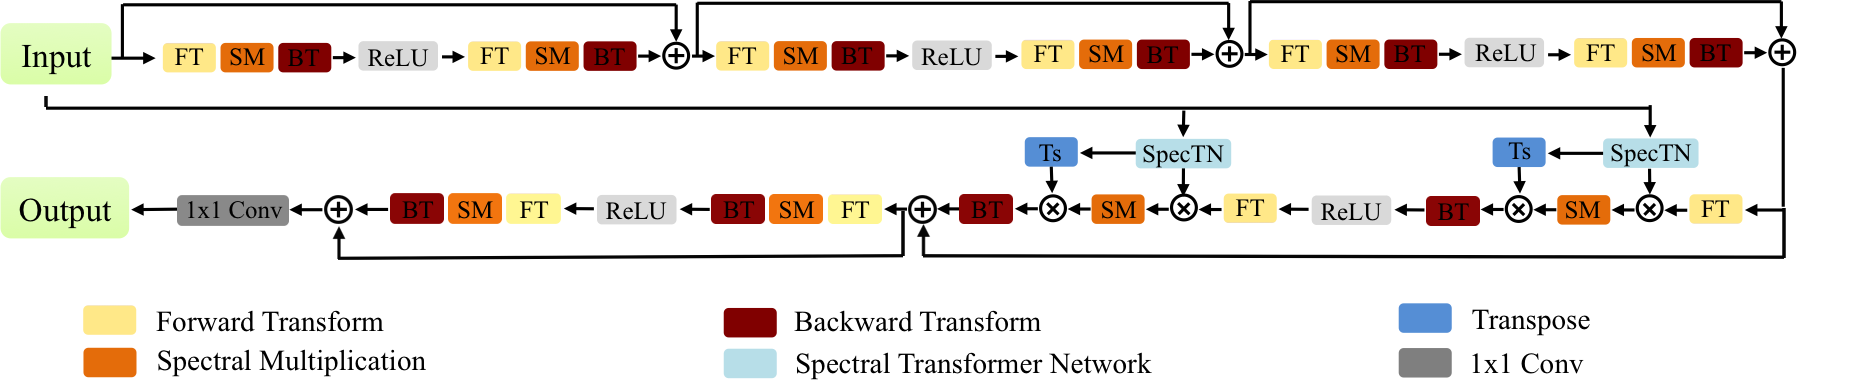
\includegraphics[width=0.9\linewidth]{./fig/architecture_v3.png}
    \caption{Architecture of our SyncSpecCNN. Spectral convolution is done through first transforming graph vertex functions into their spectral representation and then pointwise modulating it with a set of multipliers. The multiplied signal is transformed back to spatial domain to perform nonlinear operations. We introduce spectral transformer network to synchronize different spectral domains and allow better parameter sharing in spectral convolution. Convolution kernels are parametrized in a dilated fashion for effective multi-scale information aggregation.}
    \label{fig:architecture}
\end{figure*}

\begin{table}[]
\centering
{\footnotesize
\begin{tabular}{@{}p{0.25\linewidth}p{0.015\linewidth}p{0.015\linewidth}p{0.015\linewidth}p{0.015\linewidth}p{0.015\linewidth}p{0.015\linewidth}p{0.017\linewidth}p{0.016\linewidth}p{0.016\linewidth}p{0.015\linewidth}}
\toprule
Layer               & 1  & 2  & 3  & 4  & 5  & 6  & 7   & 8   & 9  & 10 \\ \midrule
Dilation ($\gamma$) & 1  & 1  & 4  & 4  & 16 & 16 & 64   & 64   & 1  & 1  \\
SpecTN              & No & No & No & No & No & No & Yes & Yes & No & No \\
\#Kernel Param      & 7  & 1  & 7  & 1  & 7  & 1  & 45  & 45  & 7  & 1  \\
\#Out Channel    & c  & c  & c  & c  & 2c & 2c & 2c  & 2c  & 2c & 2c\\ \bottomrule
\end{tabular}
}
\caption{Parameters used in different layers of the architecture, including dilation parameter $\gamma$ which controls convolution kernel size, whether use spectral transformer network (SpecTN), the number of learnable parameters in convolution kernels, the number of output channels after each convolution operation.}
\label{tab:architecture}
\end{table}

In a basic convolution block, a vertex function $f$ defined on $\graph$ is first transformed into its spectral representation $\myvec{\alpha}$ through Forward Transform $\myvec{\alpha} = \myvec{B}^Tf$. Then the functional map $C$ predicted by the Spectral Transformer Network will be applied to $\myvec{\alpha}$ and outputs $\myvec{\alpha}'=C\myvec{\alpha}$ for spectral domain synchronization (Sec~\ref{spectn}). A Spectral Multiplication layer is followed, pointwisely multiplying $\myvec \alpha'$ by a set of multipliers and getting $\tilde{\myvec \alpha}' = W\myvec \alpha'$, where $W$ is a diagonal matrix with its diagonal being the set of multipliers, and $\tilde{\myvec \alpha}'$ is used to denote the multiplication result. This is how we conduct convolution in the spectral domain, where spectral dilated kernels are used to capture multiscale information (Sec~\ref{sdkp}). Then we apply the inverse functional map $C_{inv}$ to $\tilde{\myvec \alpha}'$, so that we get the spectral representation $\tilde{\myvec \alpha} = C_{inv}\tilde{\myvec \alpha}'$ in the original spectral domain before canonicalization. $\tilde{\myvec \alpha}$ is then converted back to a graph vertex function through Backward Transform $\myvec \tilde{f} = \myvec{B}\tilde{\myvec \alpha}$. This building block was repeated for several times and forms the backbone of our deep architecture. We also add skip links into our SyncSpecCNN to better facilitate information flow across earlier and later layers. 
% We enforce the output $C$ of our spectral transformer network to be close to orthogonal so that its transpose $C^T$ is used as the approximated inverse functional map $C_{inv}$, as is shown in Figure~\ref{fig:architecture}. 

One interesting observation is worth mentioning: small convolution kernels correspond to smoothly transiting multipliers in the spectral domain, therefore not very sensitive to bases misalignment among shapes graphs in a certain range of spectrum and are more generalizable across graphs. As a result, we omit the spectral transformer network when the convolution kernels are small. %Moreover, while using the spectral transformer network for very large convolution kernels, instead of using our dilated parametrization, we choose to treat every single multiplier as a learnable parameter. To be specific, assuming $C\in\mathbb{R}^{k_1\times k_2}$ and transforms a subspace with dimension $k_1$ to a canonical domain with dimension $k_2$, then we will adopt a set of $k_2$ learnable parameters for spectral multiplication.

\iffalse
\todo{
\begin{itemize}
  \item Similar to conventional CNN, our SyncSpecCNN contains BatchNormalization, ReLU, DropOut, 1x1 Convolution [CITE GOOGLE INCEPTION NETWORK] layers, which are all operated in the spatial domain on graph vertex functions.
  \item Different from conventional CNN, our SyncSpecCNN conducts convolution operation on graphs through the following modules:
    \subitem Forward Transform: converts vertex functions on the graph into its spectral representation under the spectral bases. 
    \subitem Backward Transform: converts the spectral representation back to vertex functions.
    \subitem Spectral Multiplication: pointwise multiplies a spectral representation of a vertex function in the spectral domain. It's the counter part of the spatial domain convolution.
    \subitem Functional Map: linearly transforms the spectral representation of an input function
  \item In a basic convolution block, a vertex function on a shape graph is first transformed into its spectral representation through Forward Transform layer. Then a functional map layer is applied to the spectral representation for spectral domain synchronization (section xxx). A Spectral Multiplication layer is followed, pointwise multiplying the spectral representation by a set of multipliers. This is the part conducting convolution in the spectral domain, where spectral dilated kernels are used to capture multiscale information. Then we convert the spectral representation back to a graph vertex function through Backward Transform. This building block was repeated for several times and forms the backbone of our deep architecture.
\end{itemize}
}
\fi

\subsection{Spectral Dilated Kernel Parameterization}
\label{sdkp}
Yu et al.~\cite{yu2015multi} has proved the effectiveness of multi-scale kernels for aggregating context information at different scales in the task of image segmentation. They propose to use dilated kernels to increase the kernel size without increasing the number of parameters. We parametrize our convolution kernels in a similar flavor but in the spectral domain, which turns out to be straightforward and effective. Essentially, we find that multi-resolution analysis on graphs could be achieved without complicated hierarchical graph clustering.

Before explaining what the exact parametrization is, we first discuss the intuition behind our design. The Spectral Multiplication layer modulates the spectral representation $\myvec \alpha=\{\alpha_i\}$ by a set of multipliers from the kernel, where $\alpha_i$ is the spectral coordinate of vertex function at basis $\myvec{b}_i$. Note that $\lambda_i$ can be interpreted as the frequency of its corresponding eigenbasis $\myvec b_i$, and $\myvec b_i$ itself is a vertex function that captures the intrinsic geometry of the shape. We assume that $\lambda_i$'s are sorted ascendingly and arrange $\myvec{b}_i$'s accordingly.

The multiplers are the spectral representation of convolution kernel. Denote the set of multipliers as $\myvec m=\{m_i\}$, each corresponds to one $\lambda_i$. Regard $\myvec m$ as a function of $\lambda_i$. 

Again, generalized from conventional Fourier analysis, if $\myvec m$ is concentrated in the low-end of the spectrum, the corresponding spatial kernel function is smooth; conversely, if the corresponding spatial functions is localized, $\myvec m$ is smooth. Therefore, to obtain a smoother kernel function as in \cite{yu2015multi}, we constrain the bandwidth of $\myvec m$, enabling us to learn a smaller number of parameters; in addition, varying the smoothness of $\myvec m$ would control the kernel size. 

To be specific, we associate each Spectral Multiplication layer with a dilation parameter $\gamma$ and parameterize $m_i$ as a combination of some modulated exponential window functions, namely

\vspace{-0.25cm}
\begin{align*}
    m_i = \sum_{j=0}^n\omega_{2j+1}\text{e}^{-j\gamma \lambda_i}\text{cos}(j\gamma \lambda_i \pi)
    +\sum_{j=1}^n\omega_{2j}\text{e}^{-j\gamma \lambda_i}\text{sin}(j\gamma \lambda_i \pi)
    \vspace{-0.25cm}
\end{align*}

Here $\myvec \omega$ is a set of $2n+1$ learnable parameters, $n$ is a hyper-parameter controlling the number of learnable parameters. Large $\gamma$ corresponds to rapidly changing multipliers with small bandwidth, thus a smooth kernel with large spatial support. On the other hand, small $\gamma$ corresponds to slowly changing multipliers with large bandwidth, corresponding to kernels with small spatial support. Instead of using an exponential window only, we add $\text{sin}/\text{cos}$ modulation to increase the expressive power of the kernel. Figure~\ref{fig:kernelvis} shows a visualization of modulated exponential window function with different dilation parameter.

Our parametrization has three main advantages: First, it allows aggregating multi-scale information since the size of convolution kernels vary in different layers; Second, large kernels could be easily acquired with a compact set of parameters, which effectively increases the receptive field while mitigates overfitting; Third, reduced parameters allow more efficient computation.
\iffalse
\todo{
\begin{itemize}
  \item We use modulated exponential window to parametrize our convolution kernel in the spectral domain. 
  \item Observing that the spacial support of these kernels increase with a shrink of the exponential window width, we adapt exponential window with different width in different layers of the network. This allows the network to capture information at different spatial scales.
  \item We use cos/sin function to modulate the exponential window, which increases the expressive power of the kernel without increasing its spatial support much. 
\end{itemize}
}
\fi

\vspace{-0.1cm}
\begin{figure}
    \centering
    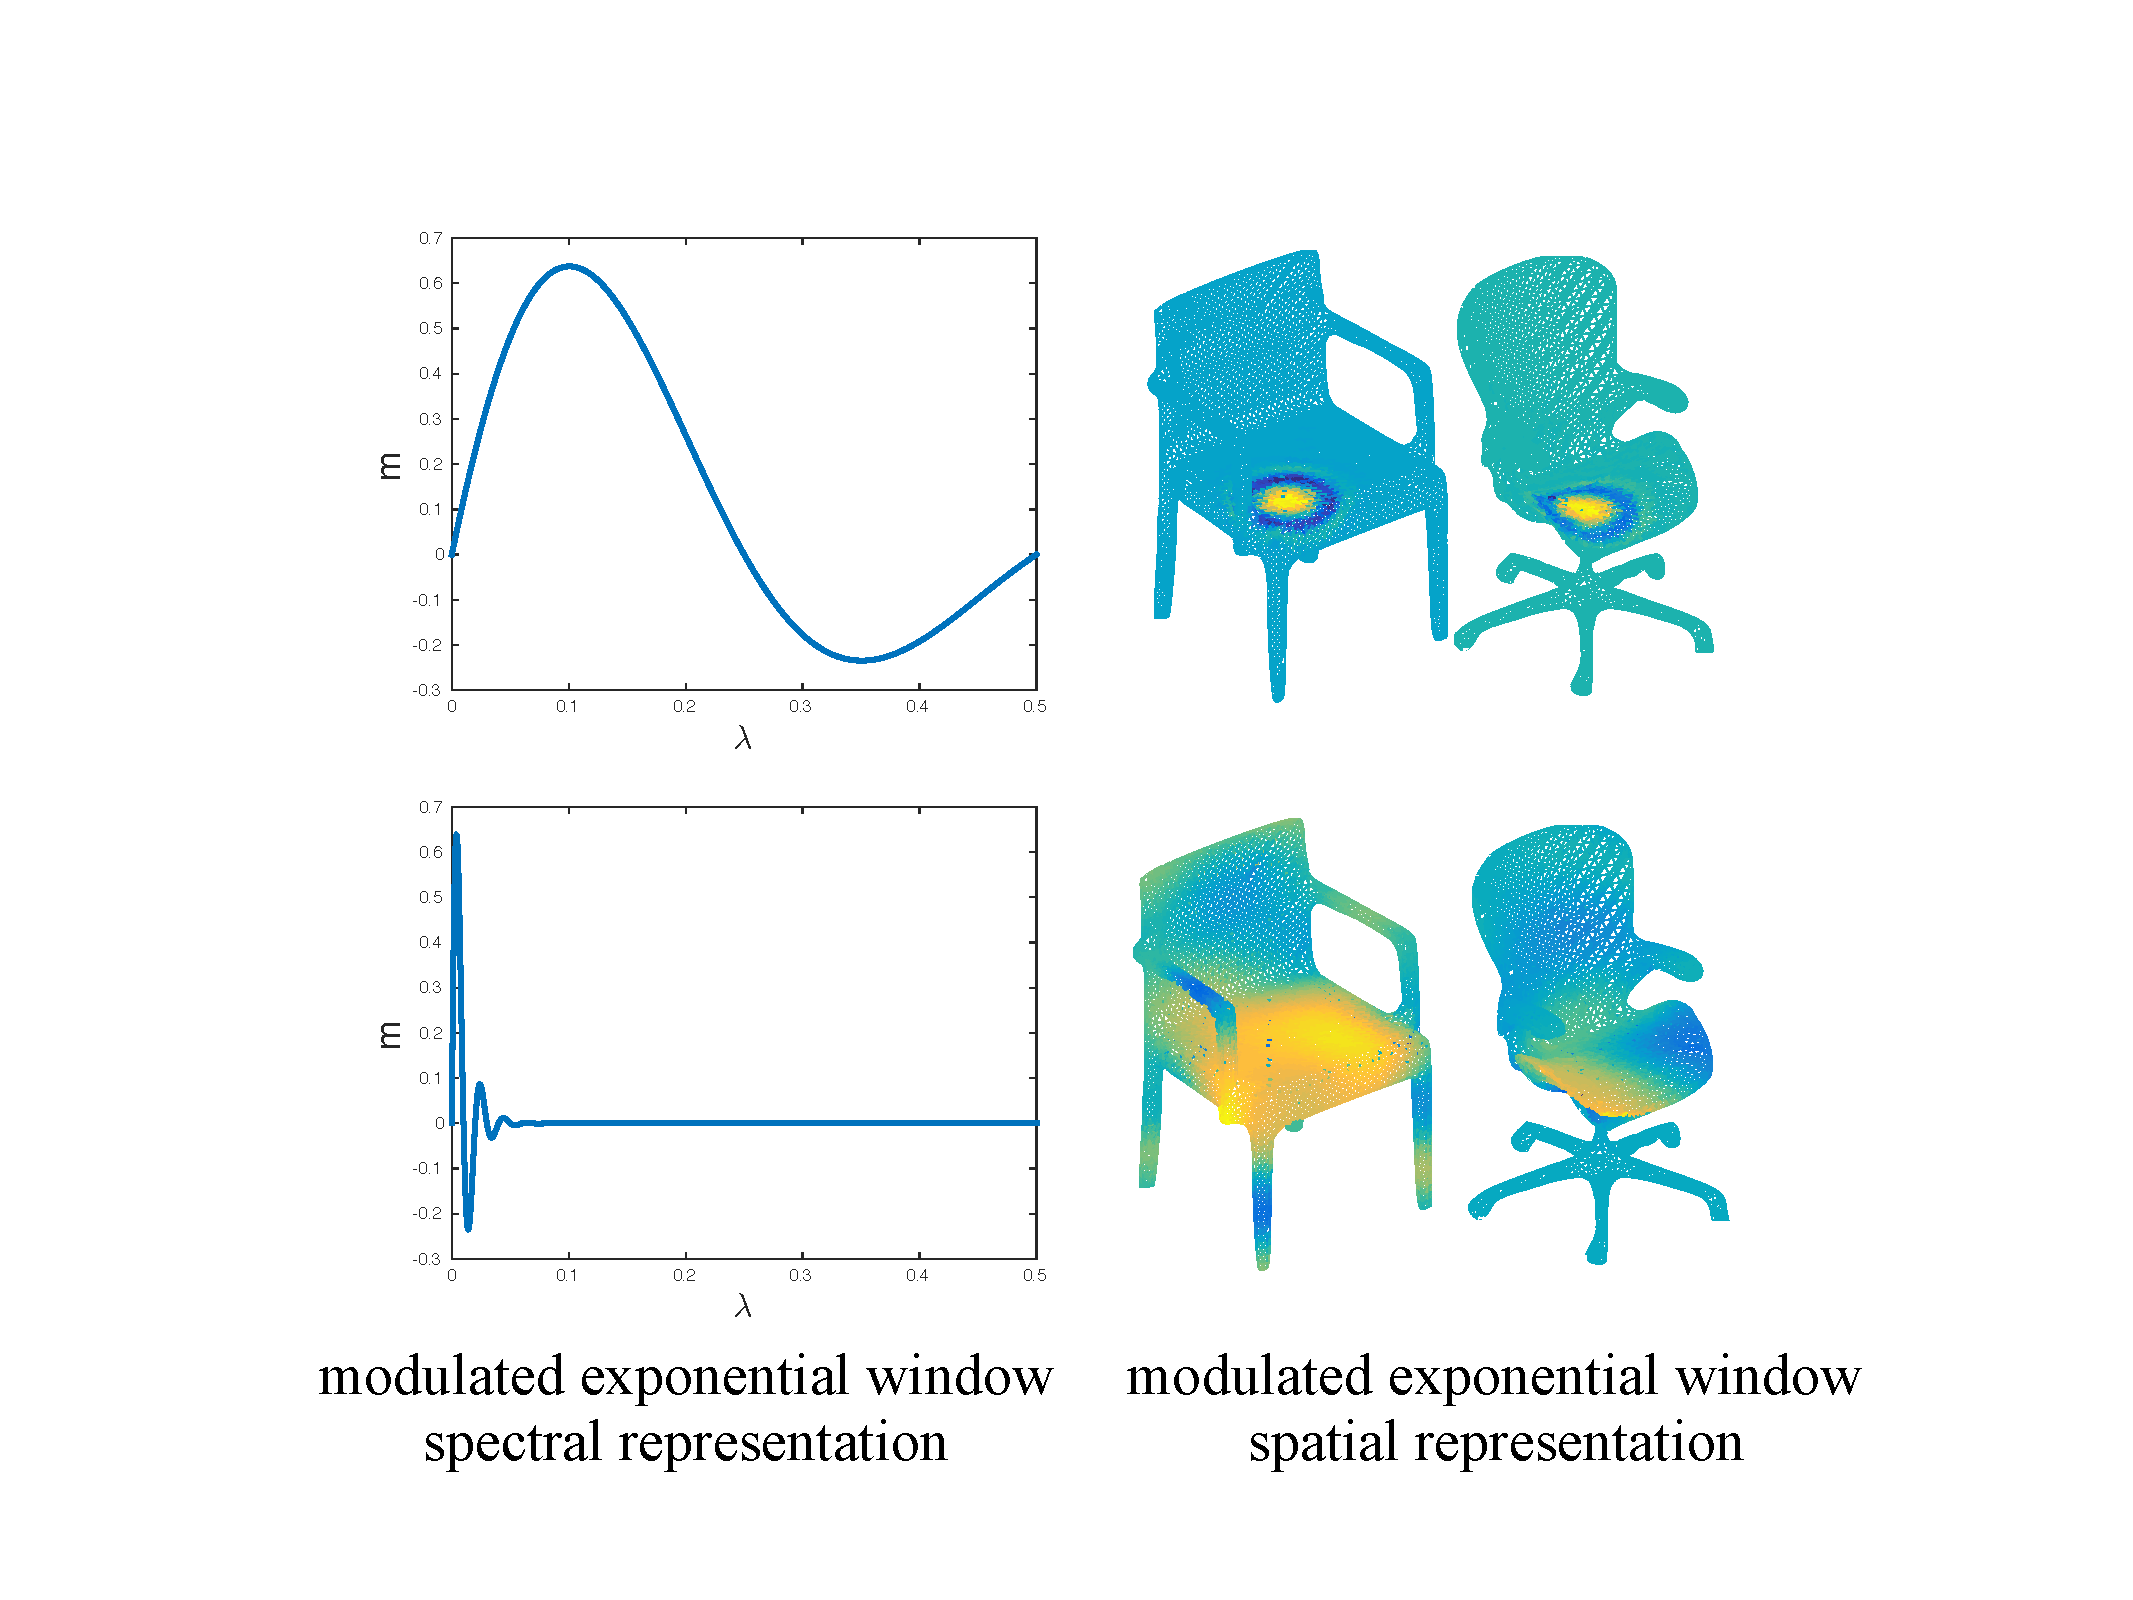
\includegraphics[width=0.8\linewidth]{./fig/kernelvis4.pdf}
    \caption{Visualization of modulated exponential window function with different dilation parameters in both spectral domain and spatial domain. The same spectral representation could induce spatially different kernel functions, especially when the kernel size is large.}
    \label{fig:kernelvis}
    \vspace{-0.3cm}
\end{figure}

\subsection{Spectral Transformer Network}
\label{spectn}
As is shown in Figure~\ref{fig:kernelvis}, the same spectral parametrization of kernels could lead to very different vertex functions when the underlying spectral domains are different. This problem is especially prominent when the kernel size is large. Therefore, being able to synchronize different spectral domains is the key to allow large kernels sharing parameters across different shape graphs. 

\subsubsection{Basic idea} According to \cite{ovsjanikov2012functional} and \cite{wang2013image}, one way to synchronize the spectral domains of a group of shapes is through a tool named functional map. In the functional map framework, one can find a linear map to pull the spectral domain of each individual shape to a canonical space, so that representations in the individual spectral domains become comparable under a canonical set of bases. Indeed, given each shape $S$, this linear map is as simple as a matrix $C$, which linearly transforms the spectral representation $\myvec \alpha$ on one shape to its counterpart $\myvec \alpha'$ in the canonical space. Note that, {\bf from the synchronization in the spectral domain, one induces a spatial correspondence on the graph, vice versa}. Viewing the spectral domain as the dual space and spatial domain on graph as the primal space, this {\bf primal-dual relationship} is the pivotal idea behind functional map.

Inspired by this idea, we design a Spectral Transformer Network (SpecTN) for the spectral domain synchronization task. Our SpecTN takes a shape $S$ as input and predicts a matrix $C$ for it (see Figure~\ref{fig:architecture}), so that
% \vspace{-0.25cm}
% \begin{align*}
$\myvec \alpha'=C \myvec \alpha$.
% \vspace{-0.25cm}
%\end{align*}
Thus, without SpecTN, $\myvec \alpha$ will be directly passed to subsequent modules of our network; with SpecTN, $\myvec \alpha'$ will be passed. In Figure~\ref{fig:jointbasis}, we show an example of how different spectral domains are synchronized after applying the linear map $C$ predicted from our SpecTN.
% The transformation is linear: $\alpha'=C\alpha$. When plugged into our SyncSpecCNN, SpecTN will learn how to actively transform the spectral domain so that the overall cost function could be minimized.

Our SpecTN draws inspiration from Spatial Transformer Network (STN)~\cite{jaderberg2015spatial}. From a high level, both SpecTN and STN are learned to align data to a canonical form.

\subsubsection{Input to SpecTN}
A proper representation for shape $\shape$ is needed as the input to our SpecTN. To allow SpecTN predicting a transform between different spectral domains, certain depiction about the underlying spectral domain is greatly helpful, i.e. graph laplacian eigenbases in our setting. In addition, since spectral synchronization couples with graph alignment, providing rough shape graph correspondences could facilitate good prediction. 

Based on these, we use voxel functions $\myvec{B}_v$ that is computed from laplacian eigenbases as the input to SpecTN:
% \vspace{-0.25cm}
% \begin{align*}
    $C=\mbox{SpecTN}(\myvec{B}_{v};\Theta).$
%     \vspace{-0.25cm}
% \end{align*} 
% As is explained soon, $\myvec{B}_v$ also implicitly provide correspondences. 
Specifically, $\myvec{B}_v$ is a \emph{volumetric reparameterization} of the graph laplacian eigenbases $\myvec{B}$, defined voxel-wise in 3D volumetric space. The volumetric reparameterization is conducted by converting graph vertex function $\myvec{B}$ into voxel function $\myvec{B}_v$ in a straightforward manner -- we simply assign a vertex function value to the voxel where the vertex lies. Since all $\myvec{B}_v$ live in the same 3D volumetric space, correspondences among them are associated accordingly.

% This representation has two merits: it depicts the underlying spectral domains of each $\shape$ through graph laplacian eigenbases; it provides rough shape correspondences for a set of spatially aligned shapes, which helps spectral alignment.

\subsubsection{Optimization of SpecTN}
Ideally, SpecTN should be learned automatically along with the minimization of the prediction loss, as the case in STN; however, in practice we find that such optimization is extremely challenging. This is because the parameters of $C$ in SpecTN is quadratic w.r.t the number of spectral bases, hundreds of times more than in the affine transformation matrix of STN. 

We address this challenge from three aspects: limit our scope to a reduced set of prominent spectral bases to curtail the parameters of $C$; add regularization to constrain the optimization space; smartly initialize SpecTN with a good starting point.  


\mypara{Reduced bases} Synchronizing the whole spectrum could be a daunting task given its high dimensionality. In particular, free parameters in $C$ grows quadratically as the dimension of spectral domain increases. To favor optimization, we adopt a natural strategy that only synchronizes the prominent part of the spectrum. In our case, the spectral parametrization of large kernels are mainly determined by the low-frequency end of the spectrum, indicating that the synchronization in this part of spectrum is sufficient. In practice, we synchronize the top $15$ bases sorted by the frequency. This idea has been verified to be effective by \cite{ovsjanikov2012functional}.

%Similar to  our SpecTN is a self-contained model that could be trained together with the end task. What's different is that STN transforms in the spatial domain whereas our SpecTN transforms in the spectral domain. This difference, however, renders a much more challenging optimization problem at training time, since the spectral alignment matrix $C$ has hundreds of of SpecTN to be rather tricky, as the 

%There are several factors differentiate SpecTN from STN. SpecTN takes a graph with vertex function as input and the input representation should be properly designed so that it is friendly to functional map prediction. Moreover, SpecTN applies a high dimensional linear transformation in the spectral space, with hundreds times more variables than STN, which makes the optimization especially tricky.

\mypara{Regularization}
Regularizations are used during training to force the output $C$ of SpecTN to be close to an orthogonal map, namely, in the overall loss function we add a term $\|CC^T-I\|_F^2$. With this regularization, $C^T$ can be used to approximate the inverse map. Such a maneuver is more friendly to differentiation and easier to train. 


 
\begin{figure}[t!]
    \centering
    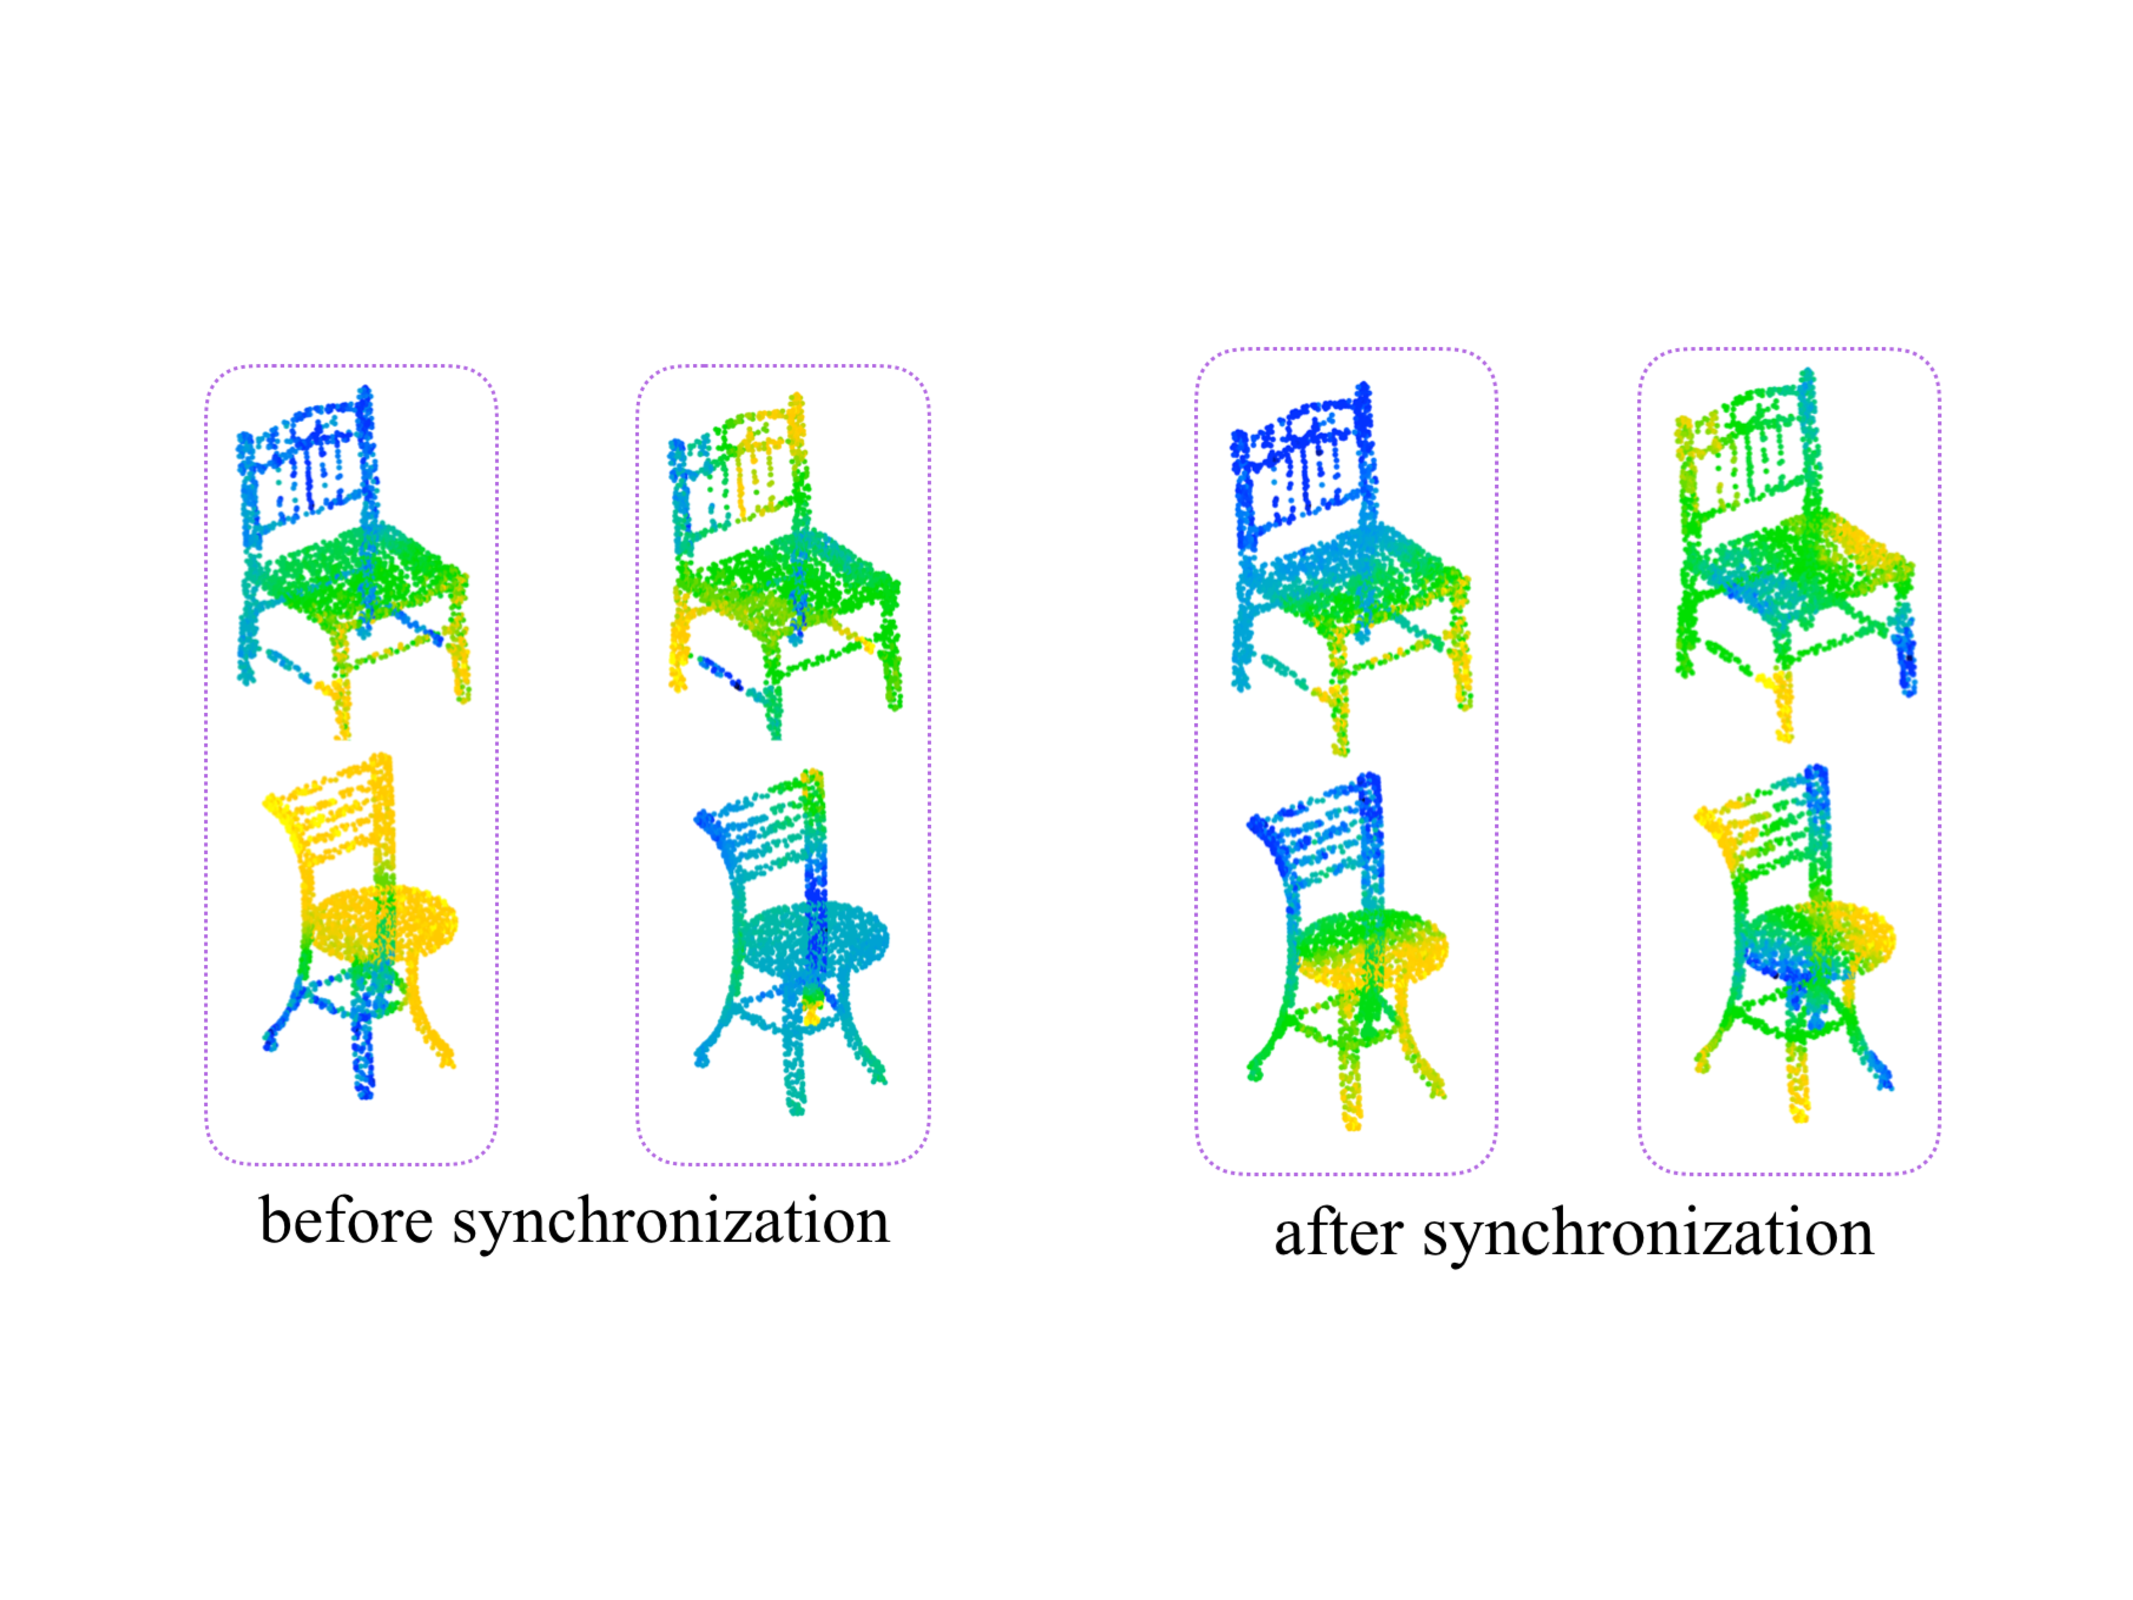
\includegraphics[width=0.4\textwidth]{./fig/visjointbasis2.pdf}
    \caption{Visualization of low frequency eigenbasis functions before and after spectral synchronization. Before synchronization, eigenbasis functions on different shapes are not aligned. After applying the transform predicted from SpecTN, different spectral domain could be synchronized and the eigenbasis functions align.}
    \label{fig:jointbasis}
\end{figure}
%Eigenbasis functions are sorted according to their frequency and same ordered functions are shown in a column.

\mypara{Initialization by precomputed functional map} 
Given the huge optimization space and the non-convex objective, a good starting point helps to avoid optimization from getting stuck in bad local minima. As stated above, our linear transformation $C$ can be interpreted as a functional map; therefore, it is natural for us to initialize $C$ accordingly and then refine it to better serve the end-task. To this end, we first precompute a set of function maps $C_{pre}$ for each shape by an external routine, which roughly align each individual spectral domain of $\shape$ to a canonical domain. Then we pretrain the SpecTN separately in a supervised manner:
\begin{equation*}
\begin{aligned}
\underset{\Theta}{\mbox{minimize}} & &\sum_i \|\mbox{SpecTN}(\myvec{B}_{v, i};\Theta) - C_{pre, i}\|^2
\end{aligned}
\end{equation*}
where $i$ indexes shapes.
This pretrained SpecTN is plugged into the  SyncSpecCNN pipeline and fine-tuned while optimizing a specific task such as shape segmentation.  Validated by our experiment, the pretraining step is crucial. 

Next we introduce how the external routine precomputes a functional map for some shape $\shape$. This functional map aligns the spectral domain of $S$ to a canonical one of an ``average'' shape $\bar{\shape}$. So we start from the construction of the ``average'' shape and then proceed to the computation of the functional map. 

The geometry of $\bar{\shape}$ is not generated explicitly. Instead, $\bar{\shape}$ is represented by its volumetric adjacency matrix $\bar{W}_v$, which depicts the connectivity of voxels in the volumetric space that all shapes are voxelized. $\bar{W}_v$ is obtained by averaging the volumetric adjacency matrices $W_v$ of all shapes. The $W_v$ for each shape $S$ is the adjacency matrix of the corresponding volumetric graph, whose vertices are all the voxels and edges indicate the adjacency of occupied voxels in the volumetric space.

The functional map $C$ from $\shape$ to $\bar{\shape}$ could be induced from the spatial correspondences between $\shape$ and $\bar{\shape}$, by the primal-dual relationship~\cite{ovsjanikov2012functional}. Since we already have the bases of $\shape$ and $\bar{\shape}$, as well as the rough spatial correspondences between them from the volumetric occupancy, this map can then be discovered by the approach proposed in \cite{ovsjanikov2012functional}. To be specific, we use $\myvec{B}_v$ to denote the volumetric reparametrization of graph laplacian eigenbases $\myvec{B}$ for each shape $\shape$, and use $\bar{\myvec{B}}_v$ to denote the grahp laplacian eigenbases of $\bar{\shape}$. $\myvec{B}_v$ and $\bar{\myvec{B}}_v$ both lie in the volumetric space and their spatial correspondence is natural to acquire. The functional map $C_{pre}$ aligning $\myvec{B_v}$ with $\bar{\myvec{B}}_v$ could be computed through simple matrix multiplication $C_{pre}=\bar{\myvec{B}}_v^T\myvec{B}_v$. The computed functional map will serve as supervision and SpecTN is pretrained to minimize the loss function $||C-C_{pre}||_F^2$.

It is worth mentioning that, if the shapes under consideration are diverse in topology and geometry, i.e. shapes from different categories, aligning every shape to a single ``average'' shape might cause unwanted distortion. Therefore we leverage multiple ``average'' shapes $\{\bar{\shape}_i\}_{i=1}^{n}$ and use a combination of their spectral domains as the canonical domain. Specifically, we assign each shape $\shape$ to its closest ``average'' shape under some global similarity measurement (i.e. lightfield descriptor) and use $\{a_i\}_{i=1}^n$ to represent such assignment, namely $a_i=1$ if $\shape$ is assigned to $\bar{\shape}_i$ and $a_i=0$ otherwise. Also we use $\bar{\myvec{B}}_{vi}$ to denote the spectral bases of $\bar{\shape}_i$. Then the functional map $C_{pre}$ for each shape $\shape$ could be computed through $C_{pre}=[a_1\bar{\myvec{B}}_{v1} \;a_2\bar{\myvec{B}}_{v2}\; ...\; a_n\bar{\myvec{B}}_{vn}]^T\myvec{B}_v$. The SpecTN is pretrained to predict a functional map which only synchronizes spectral domain of each shape to its most similar ``average'' shape.

%For more details of how this map is computed and other implementation details of our framework, please refer to our supplementary. % to the voxel function space, spanned by $\bar{\myvec{B}}_v$, where $\myvec{B}$ and $\bar{\myvec{B}}_v$ denotes the laplacian eigenbases of each individual shape graph and the average shape graph respectively. This problem couples with graph alignment and requires rough spatial correspondences to solve. To acquire this, we reparametrize each $\myvec{B}$ as $\myvec{B}_v$ defined in 3D volumetric space, so that the correspondences between each shape graph and the average shape graph can be obtained by a simple nearest neighbor lookup. The functional map $C_v$ aligning $\myvec{B_v}$ with $\bar{\myvec{B}}_v$ could be computed through simple matrix multiplication $C_v=\bar{\myvec{B}}_v^T\bar{\myvec{B}}_v$. The computed functional map will serve as supervision and SpecTN is pretrained to minimize the loss function $||C-C_v||_F^2$.
 
%Another thing worth mentioning, when the shapes under consideration are very diverse, i.e. shapes from different categories, aligning every shape to a single "average" shape might cause unwanted distortion. Therefore we leverage multiple "average" shapes and use a combination of their spectral domains as the canonical domain. The SpecTN is pretrained to predict a functional map which only synchronizes spectral domain of each shape based on its most similar "average" shape.

%For implementation details of our pipeline, we refer the reader to supplementary for details.

\iffalse
\todo{
\begin{itemize}
  \item laplacian bases from different shape graphs vary but are still roughly aligned regarding to the low/high frequency in the spectrum.
  \item small convolution kernels in the spatial domain corresponds to smooth and flatly changing spectral multipliers, which are not sensitive to bases change within a relatively wide spectrum range. Thus generalizability is not a prominent problem for small convolution kernels.
  \item large convolution kernels, on the other hand, corresponds to rapidly changing spectral multipliers, therefore very sensitive to bases change. Spectral domain synchronization becomes a key issue for across graph deep learning.
  \item in our setting, large convolution kernels are constructed by low frequency bases. Therefore we don't need to synchronize the whole spectrum of different shape graphs but only the low frequency end.
  \item we use a functional map to transform spectral representation under different shape graphs into a canonical domain, allowing parameter sharing.
  \item to learn the functional map, which is shape dependent, we design a Spectral Transformer Network, which takes the volumetric representation of each shape as input and predicts a functional map for it. The volumetric representation is not just a binary occupancy grid. Voxel cells are also equipped with spectral bases function, which can be obtained by max pooling the vertex function values falling in each voxel cell.
\end{itemize}
}
\fi

\subsection{Implementation Details}
\label{sec:impl}
In most of our experiments, input shapes are represented as point cloud with around $2000-3000$ points. Given an input shape point cloud, we build a k-nearest neighbor graph $\graph$ first. We use $k=6$ in all our experiments. Then a graph weight matrix $W$ could be constructed in which $W_{i,j}=\frac{1}{d_{i,j}^2}$ if point $i$ and $j$ are connected, $0$ otherwise. We then compute the symmetric normalized graph laplacian $L$ as $L=I-D^{-1/2}WD^{-1/2}$, where $D$ is the degree matrix and $I$ denotes identity matrix. Since many natural functions we care about could be depicted by a small number of low-frequency laplacian eigenbases, we compute and use the smallest $100$ eigenvalues as well as the corresponding eigenbases for each $L$ in all our experiments. 

The choice of dilation parameters $\gamma$, number of output channels after each convolution layer, number of learnable parameters in each convolution kernel are shown in Table~\ref{tab:architecture}. We choose $c=50$ in all of our experiments. As is mentioned, we only consider the problem of synchronizing the low-frequency end of different spectral domains, so we choose to predict a functional map $C\in\mathbb{R}^{15\times45}$ in our experiments, which maps the first $15$ eigenbases of each individual spectral domain into a canonical domain of dimension $45$. Notice the dimension of canonical domain is larger that each individual domain to allow very different shapes to be mapped into different subspaces.

%\subsection{Implementation details}
%In most of our experiments, input shapes are represented as point cloud with around $2000-3000$ points. We build k-nearest neighbor graph $\graph$ for each shape, construct its normalized graph laplacian $L$, compute and use the smallest $100$ eigenvalues as well as the corresponding eigenbases of $L$ in all our experiments. The choice of dilation parameters $\gamma$, number of output channels after each convolution layer, number of learnable parameters in each convolution kernel are shown in Table~\ref{tab:architecture}. We choose $c=50$ in most of our experiments. We refer the reader to supplementary for more details.

%In most of our experiments, input shapes are represented as point cloud with around $2000-3000$ points. Given an input shape point cloud, we build a k-nearest neighbor graph $\graph$ first. We use $k=6$ in all our experiments. Then an graph weight matrix $W$ could be constructed where $W_{i,j}=\frac{1}{d_{i,j}^2}$ if point $i$ and $j$ are connected, $0$ otherwise. We then compute the symmetric normalized graph laplacian $L$ as $L=I-D^{-1/2}WD^{-1/2}$ where $D$ is the degree matrix and $I$ denotes identity matrix. Since most natural functions we care about could be depicted by a small number of low-frequency laplacian eigenbases, we compute and use the smallest $100$ eigenvalues as well as the corresponding eigenbases for each $L$ in all our experiments. The choice of dilation parameters $\gamma$, number of output channels after each convolution layer, number of learnable parameters in each convolution kernel are shown in Table~\ref{tab:architecture}. We choose $c=50$ in most of our experiments. As is mentioned, we only consider the problem of synchronizing low-frequency end of different spectral domains, so we choose to predict a functional map $C\in\mathbb{R}^{15\times45}$ in all our experiments, which maps the first $15$ eigenbases of each individual spectral domain into a canonical domain of dimension $45$. Notice the dimension of canonical domain is larger that each individual domain to allow very different shapes mapped into different subspaces.

\iffalse
\todo{
  \begin{itemize}
    \item how to build the shape graph; compute the normalized laplacian
  \end{itemize}
}
\fi